\chapter{The IceCube Detector}
The low cross section of neutrinos is a challenge for experimentalists.
There exist two avenues for the meausrement of neutrinos.
The precise measurements of individual events, used most notably in the OPERA \cite{Description-OPERA} and DONUT \cite{DONUT-2001} to identify individual events, gives unique constraining power with low backgrounds.
More common, however, is the use of large experimental volumes to collect high-statistics neutrino samples.
For the study of atmospheric neutrinos, volumes on the order of a kiloton are required. 

The IceCube Neutrino Observatory is currently the largest neutrino detector in the world, encompassing a volume of 1 km$^3$ of glacial ice at the geographic south pole.
The design of the IceCube detector is also presented in this chapter, beginning with a description of the DOMs that make up the primary detectors within the IceCube observatory (Section~\ref{sec:dom}).
The overall geometry of the detector is discussed in Section~\ref{sec:geometry} with a focus on the differences between the larger IceCube detector and the DeepCore subarray used for oscilation searches.

\label{sec:dom}
\section{The DOM: The Basic Unit of IceCube}

\label{subsec:pmt}
\subsection{The Photomultiplier Tube}
\findref{cite https://arxiv.org/abs/1612.05093 over and over and over and over ad infinitum}
The basic unit of the IceCube detector is the \textbf{digital optical module}, often referred to simply as the \textbf{DOM}.
The DOM is designed around a downward-facing 10 inch R7081-02 photomultiplier tube (\textbf{PMT}) from Hammamatsu Photonics. \findref{https://www.sciencedirect.com/science/article/pii/S0168900210006662?via\%3Dihub (remove the backslash in the latex code if pasting the link)}\findref{probably also the hammamatsu documentation http://icecube.wisc.edu/~kitamura/NK/PMT/031112\%20R7081-02\%20data\%20sheet.pdf} and includes onboard electronics for standard operation. 
Circuit boards are included for data acquisition, control, calibration, comminuications and power conversion as well as for high voltage input from the surface.
The electronics of the DOM are encased in a spherical glass housing designed to withstand the high pressures associated with operation in the glacier of Antarctica.
The PMT is optically coupled to the glass housing in order to minimize distortion of incoming light. \findref{something about the gel?}

\needfig{steal figure 3 from the detector paper showing the DOM layout}

\needfig{also grab figure 5 from https://arxiv.org/pdf/1612.05093.pdf for the next section}

A discriminator onboard the DOM is used to identify signals from the PMT with a voltage threshold corresponding to 0.25 photoelectrons.
Each discriminator crossing begins a \textbf{DOM launch}, the lowest level signal available in the IceCube detector containing a digitization of a raw PMT output in the form of a \textbf{waveform}.
Information from the PMT is digitized using the fast analog-to-digital converter (\textbf{fADC}), which provides binned information at 40 megasamples/second for for the 6.4 microseconds following the initial DOM launch.
Simultaneously, the analog signal is recorded by the onboard custom integrated circuits known as \textbf{Analog Transient Waveform Digitizers} (\textbf{ATWDs}) for possible high quality digitization.
Launches are recorded in DOM memory while awaiting a decision from the triggering system.

\label{subsec:LC}
\subsection{Local Coincidence}
If any of the notified DOMs also record a launch within a configurable 1 microsecond window, both launches are said to form a \textbf{hard local coincidence} (\textbf{HLC}) pair.
Nearby DOMs, here defined to be either of the two DOMs above or below the current DOM, are notified of the launch via a signal sent using the \textbf{local coincidence} wiring.
In this situation, all DOMs participating in the HLC begin producing higher quality digitizations from the recorded analog signals using the ATWDs.
Launches which fail to satisfy the local coincidence conditions are referred to as \textbf{soft local coincidence} (\textbf{SLC}) hits.
Launches digitized as part of an HLC pair receive a flag. 
This flag may be used to later identify only those launches which satisfy the local coincident conditions, providing a simple, default method of identifying hits likely to be caused by particle interactions in the detector.

\label{subsec:digitization}
\subsection{Digitization}
Signals from the PMT are digitized using a variety of digitizers.
Each DOM contains two ATWD chips, each of which has access to three amplifier gain levels in order to cover the dynamic range of the PMT.
The highest gain channel is used for most pulses, although lower gains are used in cases of particularly large pulses in order to avoid loss of information due to saturation of the channel.
The ATWD chips sample the waveform at a rate of 300 megasamples/second with 128 samples per launch, recording a total of 427 nanoseconds.
A 10 meter long delay line embedded in the circuitry of the DOM allows the ATWD to record signals from approximately 75 nanoseconds before the discriminator crossing.

When digitizing a signal, the ATWD chip experiences 29 microseconds of deadtime. \findref{https://arxiv.org/abs/0810.4930}
During this time, the secondary ATWD is available to record further pulses, resulting in a total average fractional deadtime per DOM of $\mathtt{2.2 \times 10^{-5}}$ seconds/second.

Examples of digitized waveforms from the ATWD and fADC are shown in \needfig{figure 6 of https://arxiv.org/pdf/1612.05093.pdf}.
Digitized versions of the waveforms are transmitted from the DOM to the IceCube physics data acquisition system (\textbf{pDAQ}) for use in trigger and event building.


\label{sec:geometry}
\label{sec:geometry}
\section{The Geometry of the Detector}
The IceCube detector is located at the geographic south pole in Antarctica.
The Antarctic glacier forms a 3 km deep surface of clear ice over the bedrock.
IceCube uses the Antarctic glacier as both a support structure and as a detection medium for Cherenkov radiation.

\begin{figure}
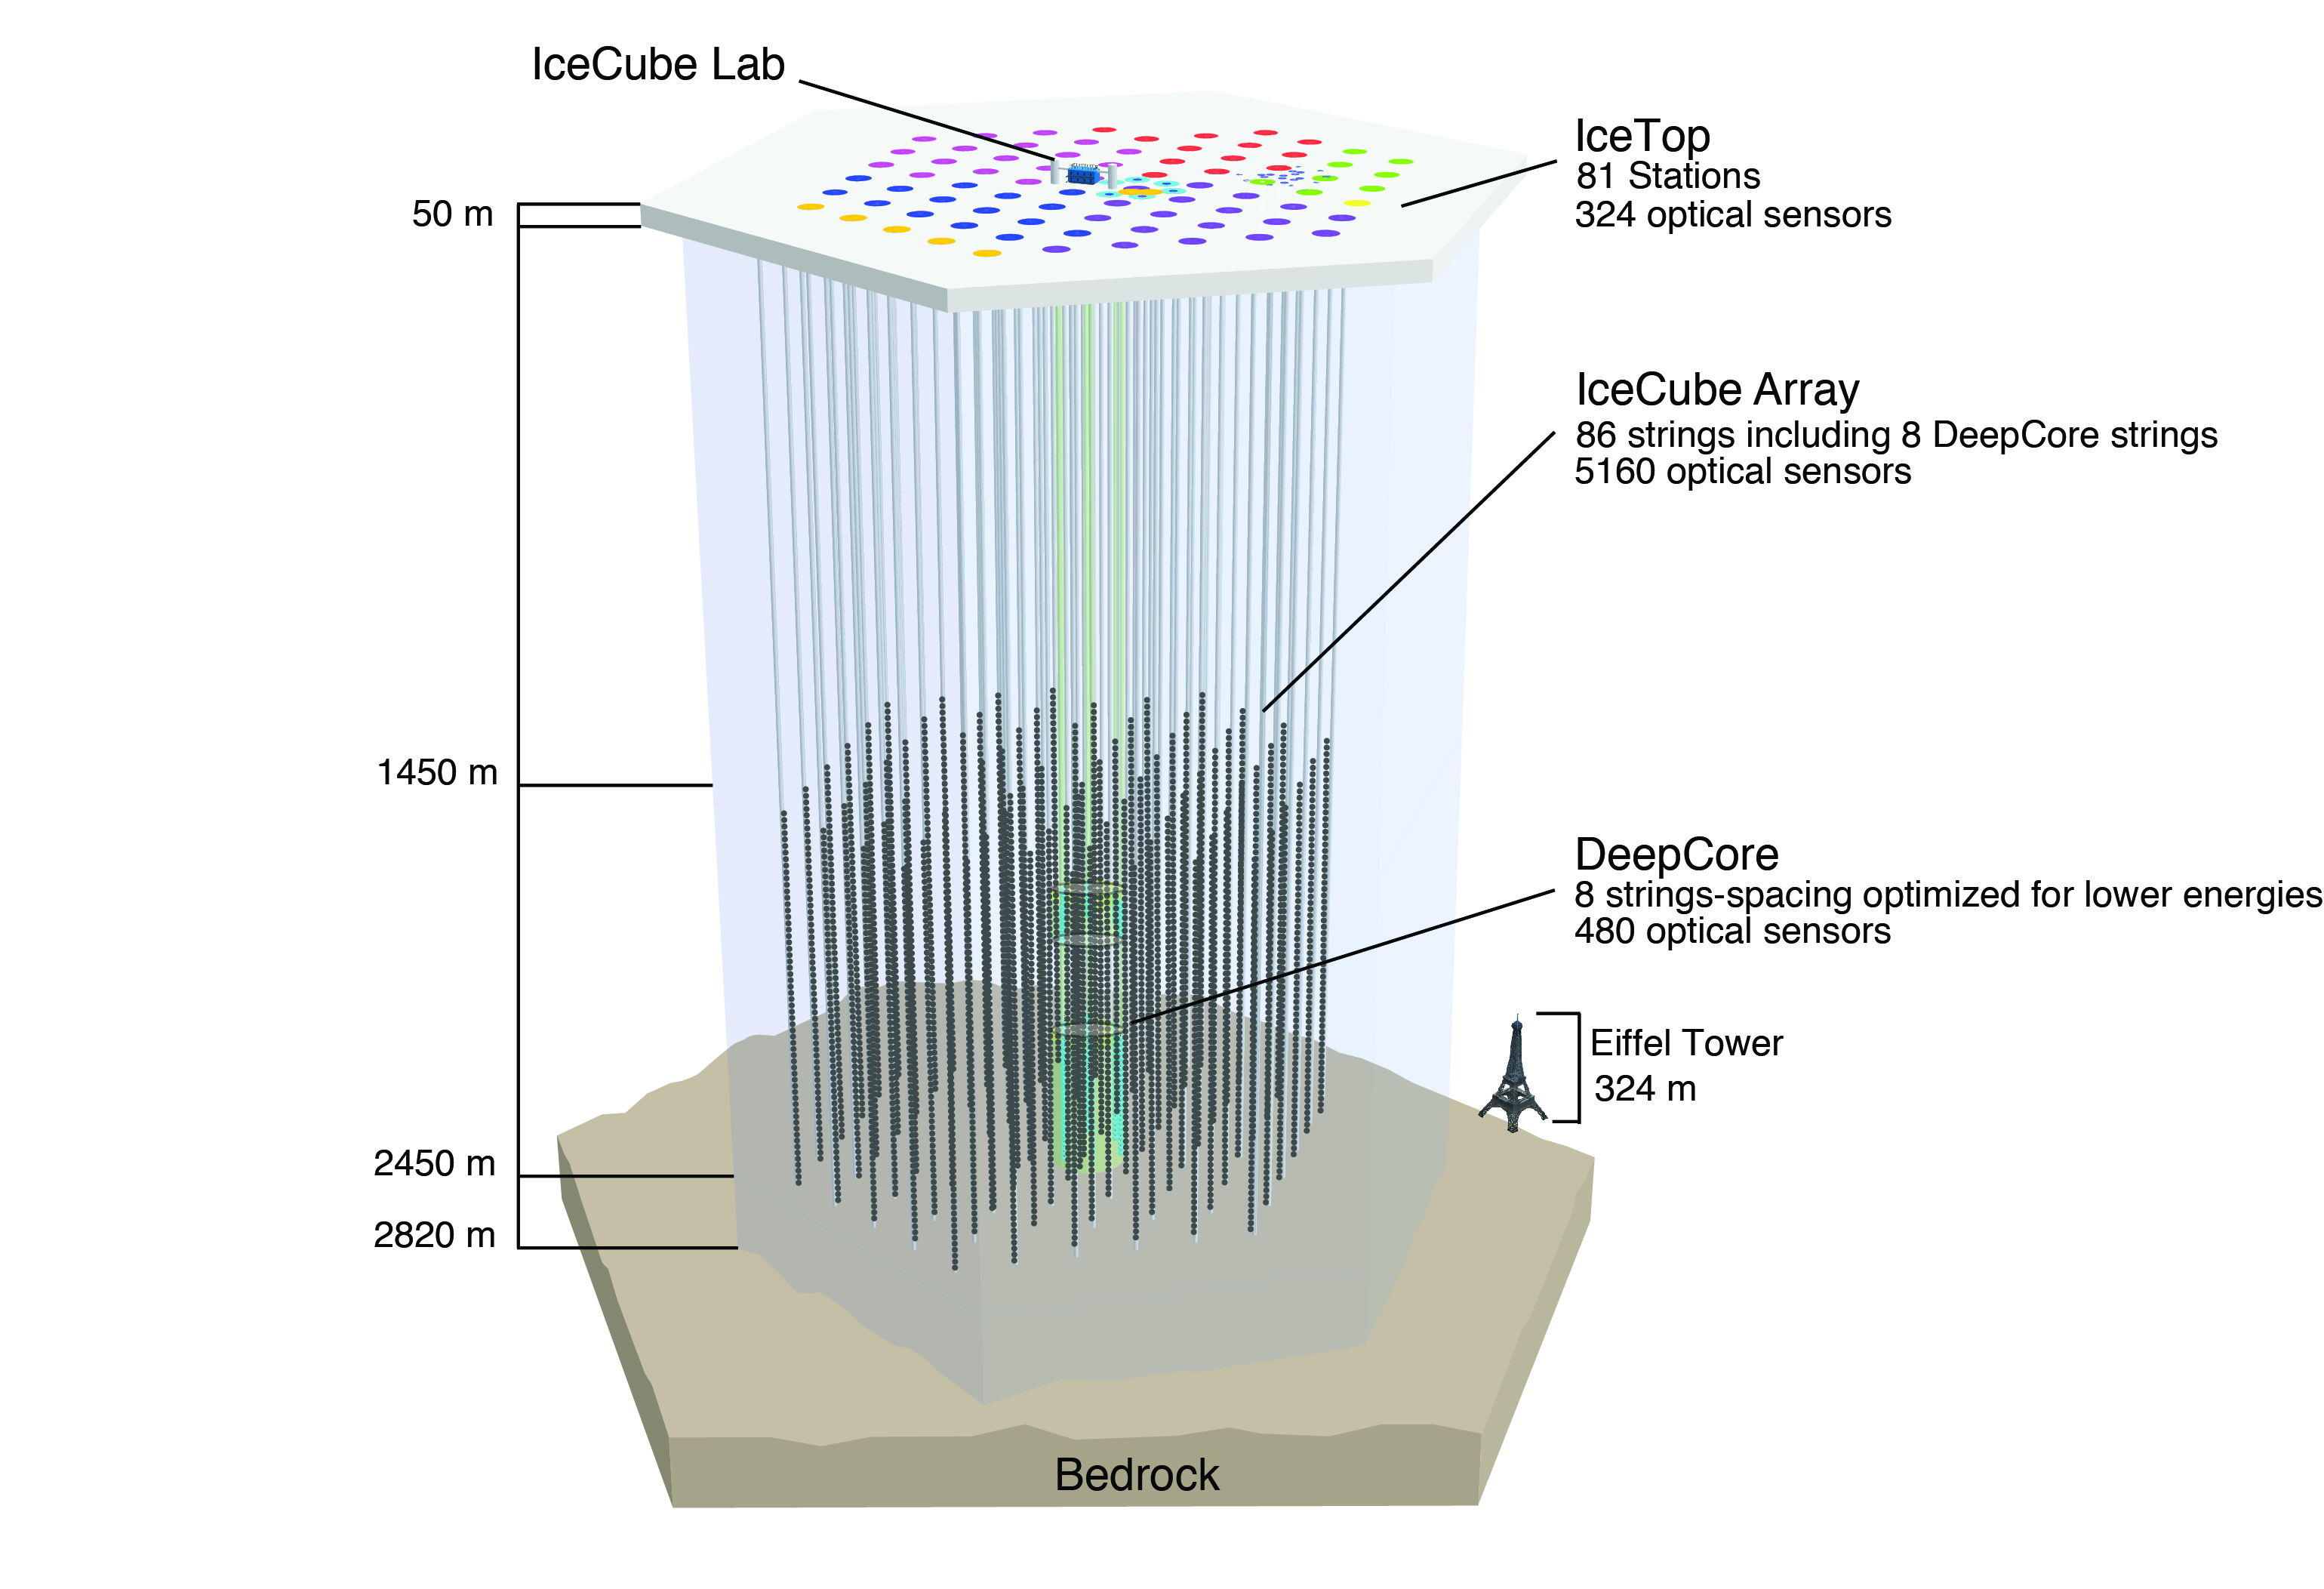
\includegraphics[width=0.9\linewidth]{ArrayWSeasonsLabels.jpg}
\caption{The IceCube Neutrino Observatory. Three separate subdetectors are shown: IceTop, a cosmic ray air shower detector; IceCube, an array designed to search for astrophysical neutrinos; and DeepCore, a dense subarray optimized for atmospheric oscillation physics measurements. The detector was deployed over multiple years. Strings deployed in the same year are shown with identical colors at the surface. }
\label{fig:icecube_depth}
\end{figure}

The IceCube observatory consists of three distinct subarrays, shown in Figure~\ref{fig:icecube_depth}, each optimized for separate physics measurements.
A total of 5160 DOMs make up the IceCube in-ice array with an additional 324 DOMs used at the surface in the IceTop air shower array \cite{Description-IceCube}.
IceCube DOMs are deployed at depths between 1450 m and 2450 m below the surface to shield the detector from atmospheric background muons.
The DOMs are deployed in a hexagonal grid in a series of 86 \emph{strings}, each of which provides connections and support for 60 DOMs.
Strings are spaced approximately 125 m apart with DOMs space 17 m apart on each string.
Each DOM in the IceCube detector is assigned a unique string number (1-86) and DOM number (1-60).

\begin{figure}
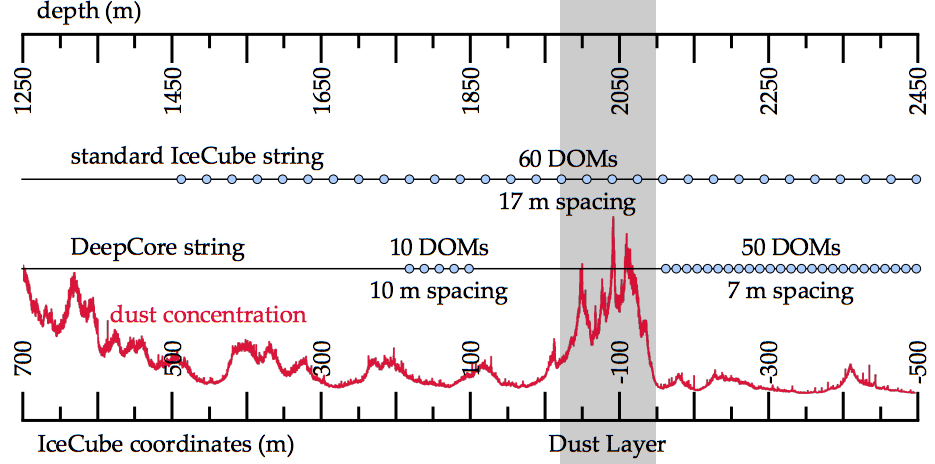
\includegraphics[width=0.9\linewidth]{icecube_depth.png}
\caption{A comparison of the standard IceCube string (right) to the DeepCore string (left). The IceCube string uses DOMs spaced 17 m apart while DeepCore divides the DOMs into a fiducial (bottom) and veto plug (top). The dust concentration is shown in red. The concentration of dust in the ice affects the scattering and absorption of the glacial ice.}
\label{fig:icecube_depth}
\end{figure}

Additional strings were installed in the glacier annually from 2004 until 2010 with partial detector data collected during construction.
During the final years of construction, a denser section of the detector was built, known as DeepCore \cite{Description-DeepCore}.
The DeepCore subarray consists of 8 strings equiped with high quantum efficiency PMTs 35\% more sensitive than the standard IceCube DOM \cite{IceCube-PMT}.
The DeepCore strings are split between a \emph{fiducial} volume, in which 50 DOMs are spaced 7 m apart on a string, and a \emph{veto plug} of 10 DOMS 10 m apart as shown in Figure~\ref{fig:icecube_depth}.
The DOMs in the DeepCore fiducial volume are located in the clearest ice of the detector at depths between 2100 m and 2450 m below the surface \cite{IceCube-SpiceMie}.
The veto cap, installed between 1750 and 1850 m below the surface, is used to identify background muons for DeepCore.

\label{subsec:icecube}
\subsection{IceCube: A Detector for TeV Neutrinos}
The IceCube detector is a regularly spaced hexagonal grid buried in the glacier with the proposed purpose of measuring astrophysical neutrino candidate events and identify the source of cosmic rays.
The IceCube array has an energy threshold of around 50-100 GeV with an optimal response above 1 TeV\cite{Description-DeepCore, Description-IceCube}.

In the standard IceCube detector, an SMT using all DOMs with a threshold of 8 HLC launches within 5 microseconds is typically used \cite{Description-IceCube}.
This trigger, known as \emph{SMT8} after the number of required hits, is designed for high signal efficiency at energies above 100 GeV with a minimum number of accidental triggers due to random detector noise.
The IceCube detector records an SMT8 rate of around 2100 Hz with less than 1 Hz expected from neutrino interactions.

Events at the TeV scales of the IceCube detector show well-defined topologies, as shown in Figure~\ref{fig:icecube_he_events}.
The IceCube detector has performed many measurements, including searches for sterile neutrinos \cite{IceCubeSterile-IC86-1}, anisotropy in the cosmic ray flux \cite{IceCube-CRAnisotropy}, measurements of the neutrino cross section at high energies \cite{IceCube-Xsec}, and the first discoveries of an astrophysical neutrino flux \cite{IceCube-HESE6}.

\begin{figure} 
\centering
    \subfloat[$\nu_e$ CC, $\nu$ NC]{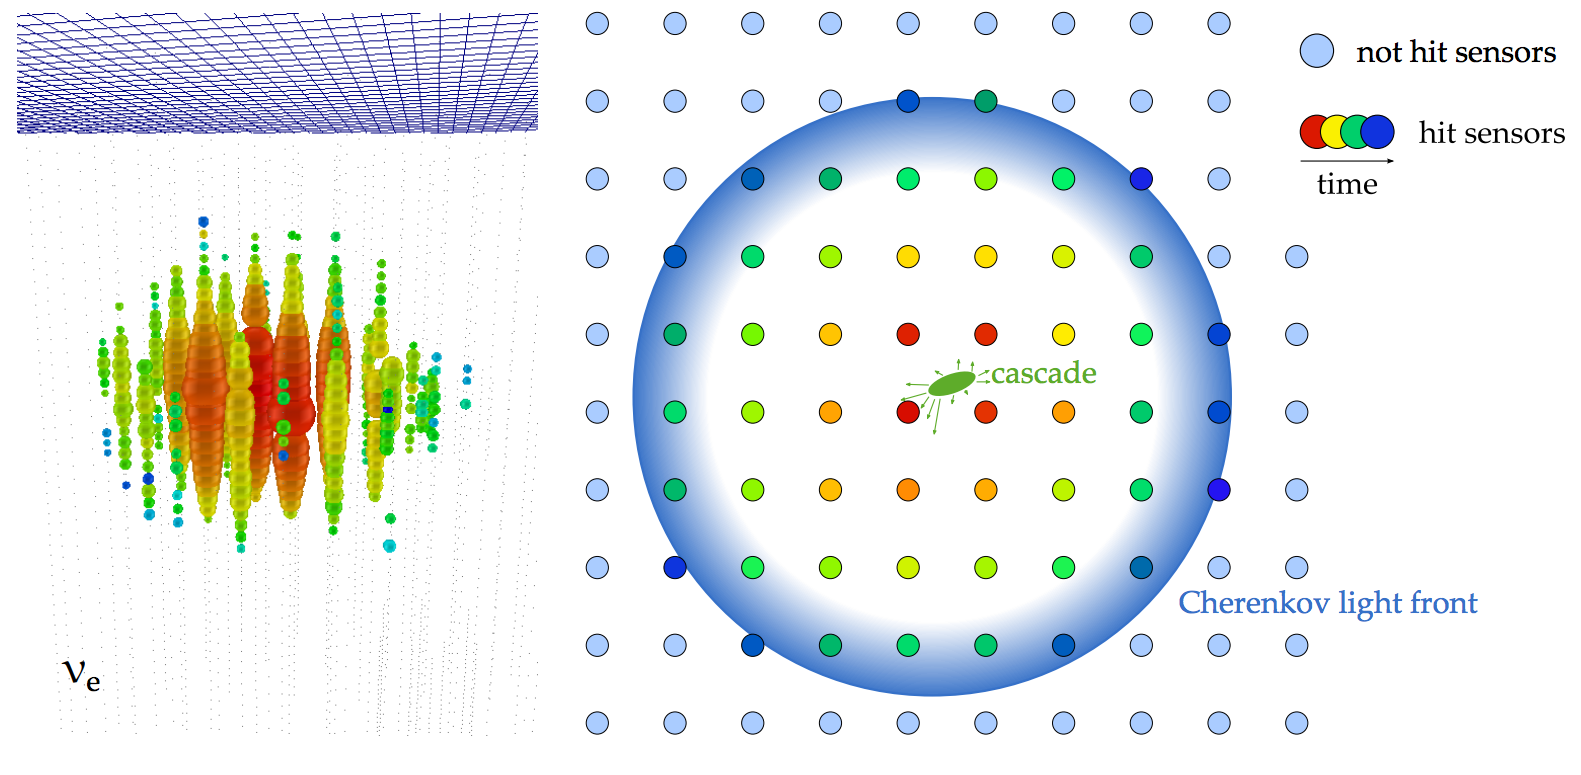
\includegraphics[width=0.7\linewidth]{icecube_he_nue.png}}
    
    \subfloat[$\nu_\mu$ CC]{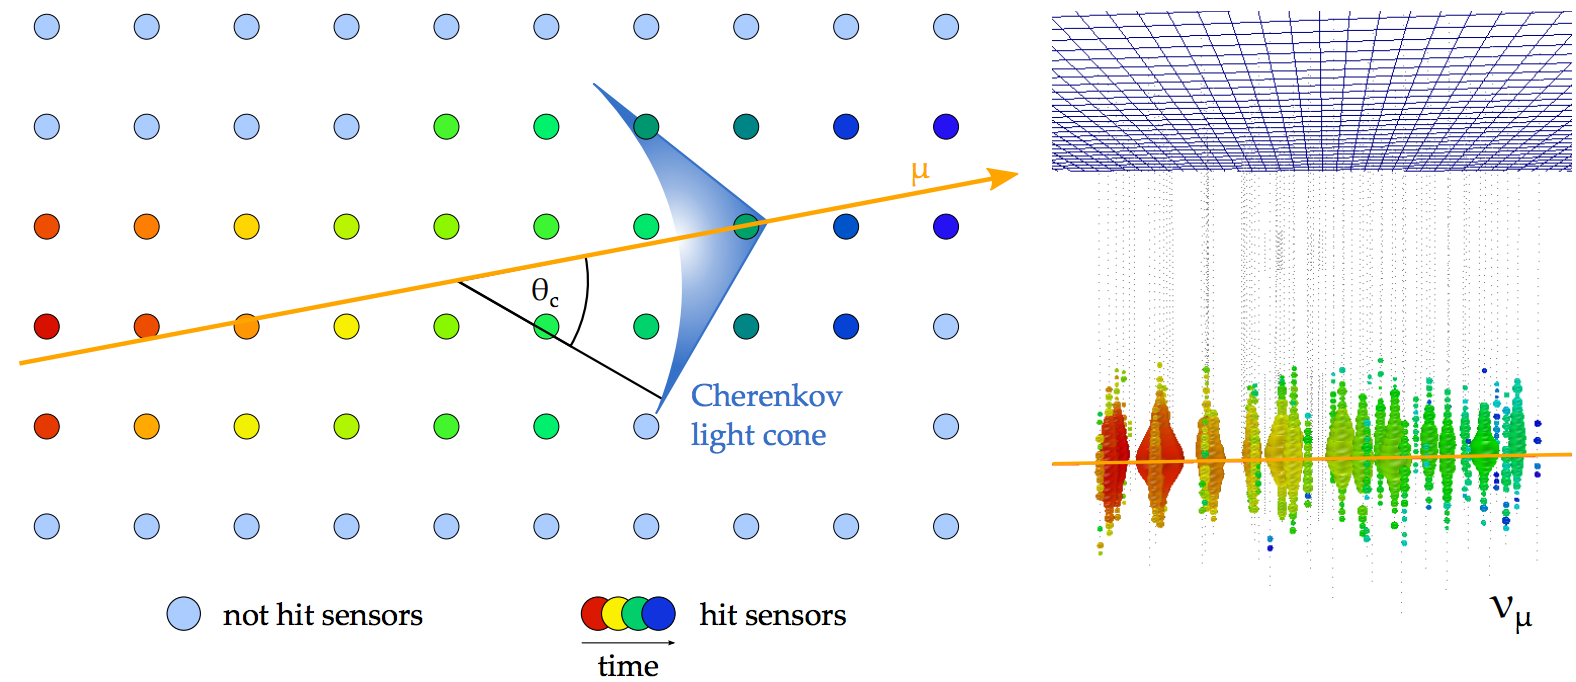
\includegraphics[width=0.7\linewidth]{icecube_he_numu.png}}
    
    \subfloat[$\nu_\tau$ CC]{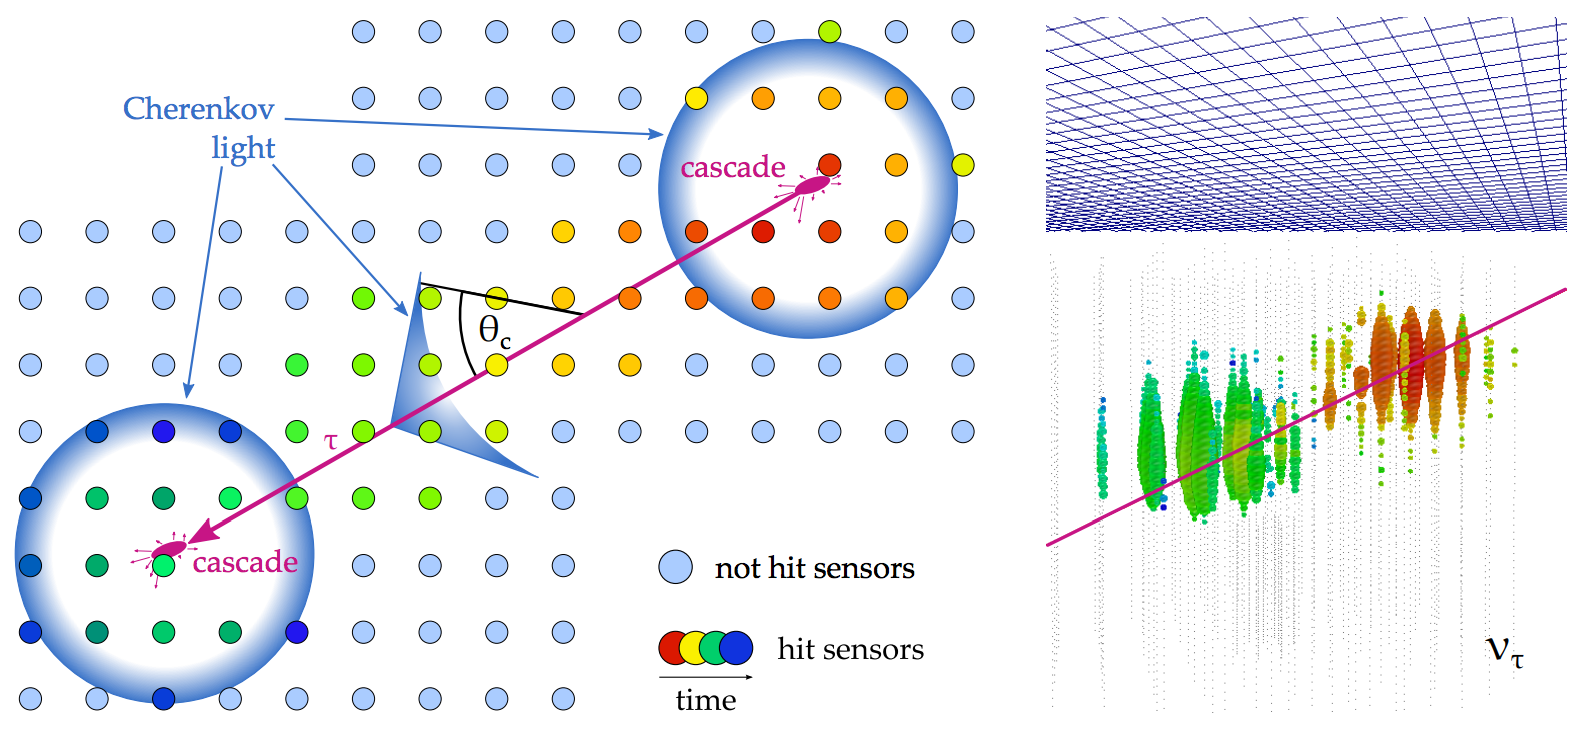
\includegraphics[width=0.7\linewidth]{icecube_he_nutau.png}} 
\caption{Examples of event topologies above 1 TeV using the full IceCube array. Event views shown in (a) and (b) are from actual events discovered by the IceCube detector \cite{IceCube-AstroNu}. Images taken from \cite{Thesis-Euler}. (a)$\nu_e$ CC and $\nu$ NC show similar behavior from electromagnetic and hadronic interactions, which result in a shower of particles that quickly scatter in the ice. Cherenkov emission from these events appears roughly spherical in the detector. These events are known as "cascades". (b) $\nu_\mu$ CC events begin with a hadronic interaction, then produce Cherenkov light from the outgoing muon. Above 1 TeV, the track of the outgoing muon becomes clearly visible. (c) Above 10 TeV, the tau lepton from a $\nu_\tau$ CC may travel a significant distance before decaying. This results in two well-separated cascades in the detector, a tell-tale signature of $\nu_\tau$ CC interactions.}
\label{fig:icecube_he_events}
\end{figure}

\label{subsec:deepcore}
\subsection{DeepCore: Extending the Reach to GeV Scales}
The DeepCore detector was designed to be a smaller, denser detector optimized for the measurement of atmospheric neutrino oscillations.
The denser spacing and clear ice of DeepCore lower the energy threshold to around 10 GeV \cite{Description-DeepCore}, permitting the study of oscillations.
DeepCore was installed at the bottom of the IceCube array near the center of the IceCube hexagonal grid.

In DeepCore, the desire for lower energy events led to the introduction of a separate trigger, known as \emph{SMT3}.
This trigger, using only DOMs within the DeepCore fiducial volume, searches for at least three HLC launches occuring within 2.5 microseconds.
This effectively lowers the triggering threshold from roughly 100 GeV with the larger IceCube array to approximately 10 GeV.
The SMT3 rate, at 250 Hz \cite{Description-IceCube, Description-DeepCore}, is substantially smaller than the SMT8 rate due to both the increased overburden as well as the smaller number of PMTs included in the SMT3 DOMSet.
By placing the detector inside of the larger IceCube array, DeepCore allows analyzers to use the IceCube detector as an active veto, reducing the background rate to 17 Hz.

DeepCore events do not show the clean topological separation of the higher energy IceCube events as seen in Figure~\ref{fig:icecube_he_events}.
Events may be separated broadly into \emph{cascade-like} and \emph{track-like} statistically using information contained in the timing of hits in the detector.
Such separation techniques are energy-dependent and do not perform well at very low energies.

\begin{figure}
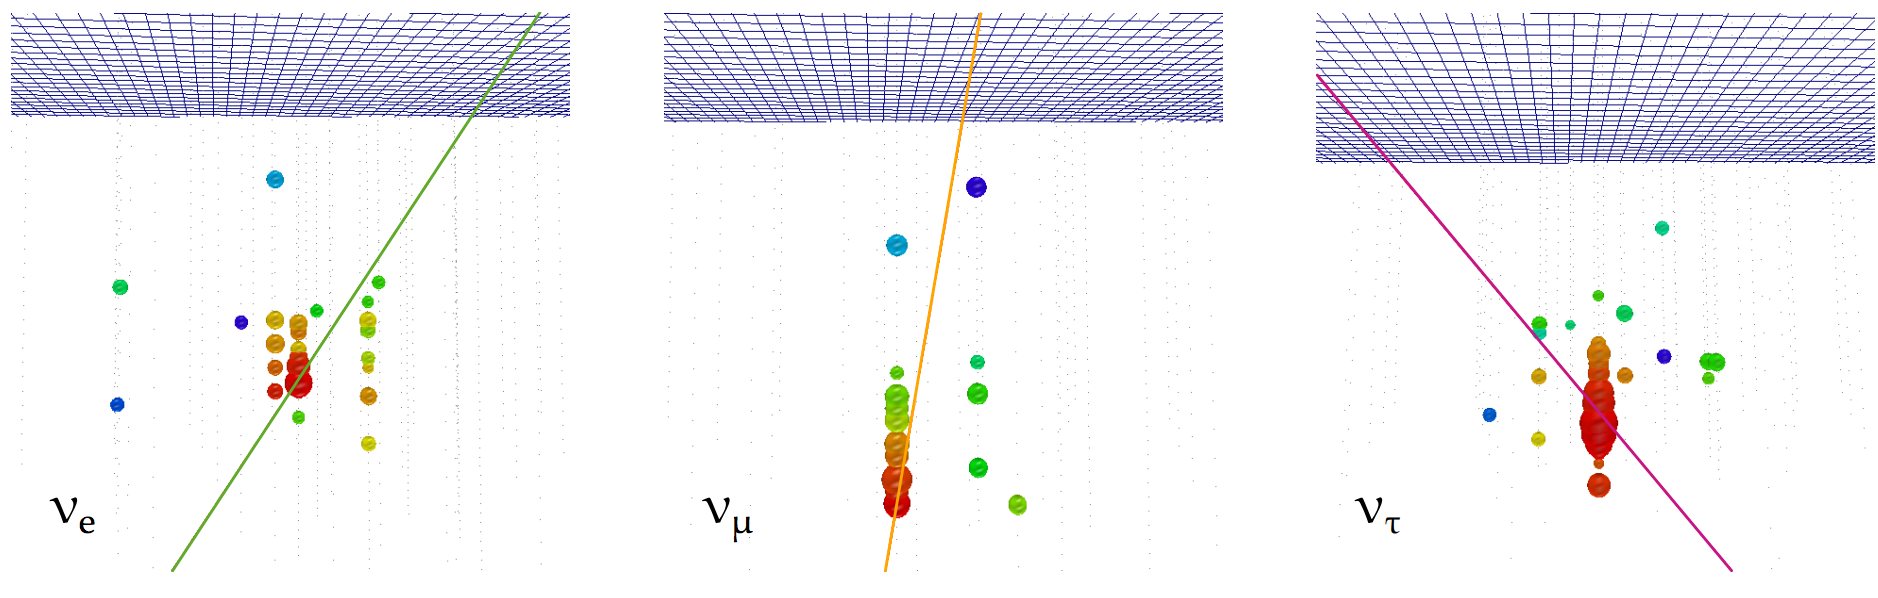
\includegraphics[width=0.9\linewidth]{deepcore_le_views.png} 
\caption{A selection of 50 GeV simulated events in DeepCore taken from \cite{Thesis-Euler}. Unlike the event topologies at high energies, DeepCore events do not show distinct event types.}
\label{fig:deepcore_events}
\end{figure}

DeepCore has observed atmospheric neutrino oscillations in the $\nu_\mu \rightarrow \nu_\tau$ in the disappearance channel \cite{IceCube-Oscillation2013,IceCube-Oscillation2015,IceCube-Oscillation2018}, with the most recent measurement showing competitive precision to dedicated measurements performed with particle accelerators.

While DeepCore was designed for oscillation physics, the neutrinos may be used for other purposes as well. 
Recent work with DeepCore has shown sensitivity to studying dark matter interactions in the sun \cite{IceCube-LE-SolarDarkMatter} and in the galaxy \cite{IceCube-LE-GalacticDarkMatter}.




\label{sec:ice}
section{Optical Properties of the Antarctic Glacier}

\label{sec:bulk_ice}
\section{The Bulk Ice Model}
The Antarctic glacier, with a thickness of 2.8 km at the geographic south pole \cite{IceCube-SpiceMie}, forms both the support structure and the interaction medium for IceCube.
During deployment, measurements of the scattering properties of the ice were taken during deployment of the IceCube strings.
The IceCube dust logger emitted laser light aimed into the undrilled ice and detected backscattered photons\cite{IceCube-DustLogger1, IceCube-DustLogger2}.
The results are shown in Figure~\ref{fig:dust_logger}

\begin{figure}[h]
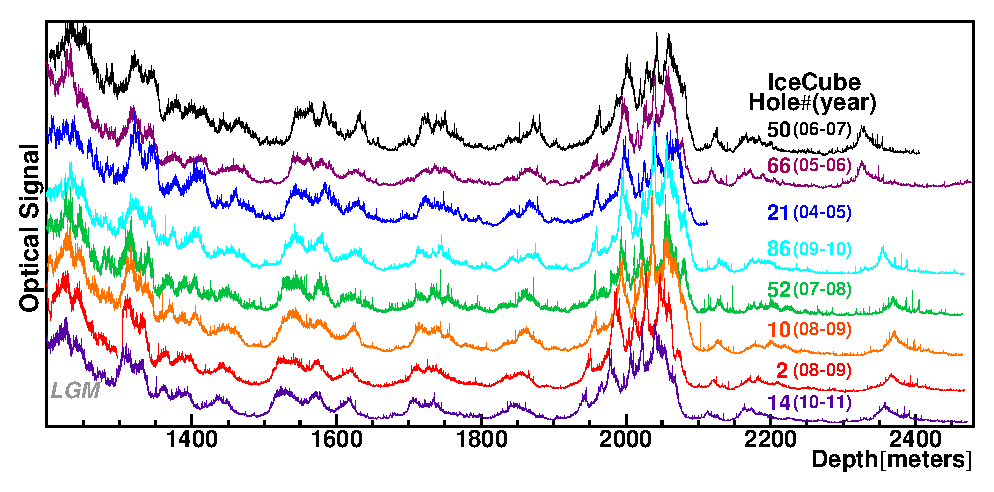
\includegraphics[width=0.9\textwidth]{dustlogger.eps} 
\caption{The data from the dust loggers deployed in various drill holes in IceCube during deployment. Data from individual holes has been offset in the y direction for clarity. Larger relative values of the "Optical Signal" represent more scattering in the ice while smaller values indicate clearer ice. The "dust layer" is visible in all drill holes around 2000 m. Deepcore DOMs are deployed below this layer. Image taken from \cite{IceCube-DustLogger-Raw}.}
\label{fig:dust_logger}
\end{figure}

Peaks are present in the dust logger data due to volcanic events in the Earth's past \cite{IceCube-DustLogger1,}.
The most significant peak, a set of features around a depth of 2000 m, form what is known as the \emph{dust layer} of IceCube, a region with significantly higher scattering and absorption properties than the surrounding ice.

To improve the modeling of the glacier, dedicated measurements have been performed using light-emitting diodes (LEDs, also known as \emph{flashers} in IceCube) onboard the DOMs \cite{IceCube-SpiceMie, Description-IceCube}.
In specialized calibration runs, the LEDs are flashed at a few Hertz for a few minutes while nearby DOMs recieve the emitted light.
Monte Carlo simulations of the flashers are used with varying ice properties in order to identify the most likely properties of the ice
Each flashing and detecting DOM pair provides a set of known times, positions, and light output in the ice, allowing for the properties of the intervening medium to be determined.

\begin{figure}[h]
\centering
\begin{tabular}[b]{c}
  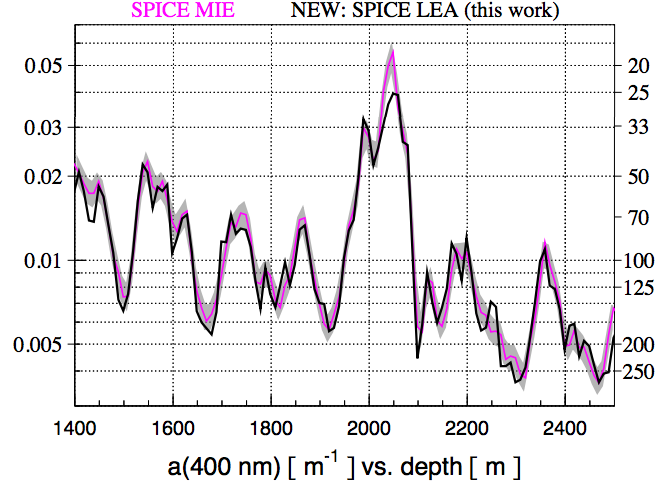
\includegraphics[width=0.45\linewidth]{absorption.png} \\
  \small (\textbf{\color{ctcolormain}a}) Absorption
\end{tabular} \hspace{2pt}
\begin{tabular}[b]{c}
  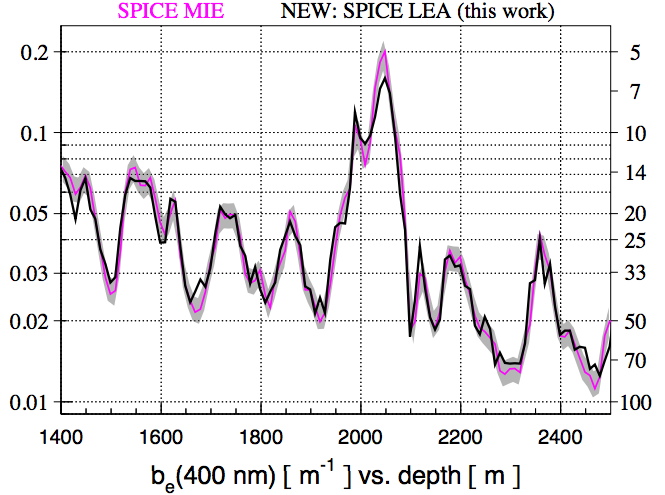
\includegraphics[width=0.45\linewidth]{scattering.png} \\
  \small (\textbf{\color{ctcolormain}b}) Scattering
\end{tabular}
\caption{The absorption and effective scattering properties of the ice as fit to flasher data. Two models are shown representing different generations of ice models used for simulation. The "Mie" model does not include anisotropy while the "Lea" model does. Figure from \cite{IceCube-SpiceLea}.}
\label{fig:spicelea}
\end{figure}

The modern ice model used for this thesis consists of three main properties: the absorption, the scattering, and the anisotropy of the ice \cite{IceCube-SpiceLea}.
The measured properties of the absorption and scattering may be seen in Figure~\ref{fig:spicelea} while the effect of the anisotropy can be seen in Figure~\ref{fig:anisotropy}.
Scattering photons change direction, losing information about the direction of the emission source.
Absorbed photons are not visible to the detector, potentially modifying the observed number of photons and the reconstructed energy of an event.
The anisotropy, consisting of a direction and magnitude, modifies the ice properties as a function of direction due to movement and compression of the glacier over time.
The anisotropy affects both the scattering and absorption from each direction in the x-y plane and can affect the azimuthal directions of reconstructions in IceCube.

\begin{figure}[h]
\centering
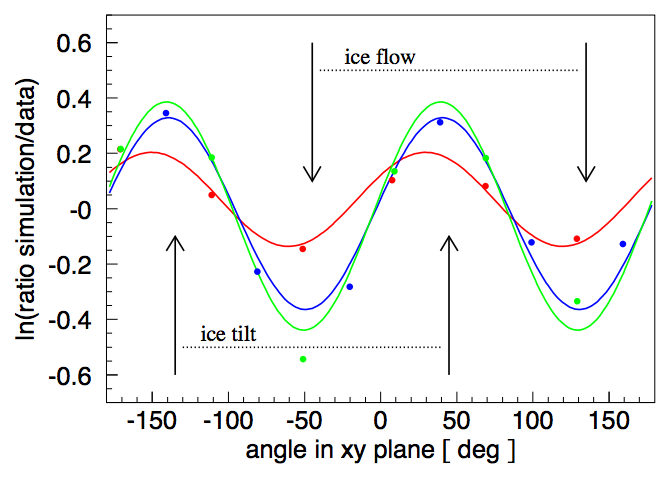
\includegraphics[width=0.6\linewidth]{anisotropy.png}
\caption{The effect of the anisotropy on the light output from a flasher on string 63. Measurements (points) are shown for receiving DOMs at three distances: at 125 m (red), at 217 m (blue), and at 250 m (green). A line is included to show the expected effect of anisotropy at each distance. The y-axis shows the ratio of a simulation of the same flasher without including anisotropy to data. A modulation is observed as a function of direction in the x-y plane.}
\label{fig:anisotropy}
\end{figure}


\label{sec:hole_ice}
\section{The Hole Ice}
After the strings were deployed, each drill hole was allowed to refreeze. 
The refrozen column of ice around each string is referred to as the \emph{hole ice}.
Using a dedicated camera deployed at the bottom of string 80, the refreezing process of the hole ice has been observed over the course of several years \cite{IceCube-SwedishCamera, Description-IceCube}.
Images\improvement{find good quality swedish camera pics?} obtained from the camera show the refrozen ice divided into three distinct regions.

The outermost region, the \emph{bulk ice}, is the original glacial ice and is unaffected by the deployment of the detector.
The outer part of the drill hole shows improved clarity compared to the bulk ice.
The central region of the drill hole, a central core of about 16 cm in diameter, shows significantly worse scattering properties than the bulk ice \cite{Description-IceCube}.
This central column, referred to as the \emph{bubble column}, affects the photon acceptance of the PMT.
Measurements to characterize the hole ice are ongoing.



